\documentclass{standalone}
\usepackage{tikz}
\usetikzlibrary{shapes.geometric}

\tikzset{
  shape example/.style= {color = black!30,
                         draw,
                         fill = yellow!30,
                         line width = .5cm,
                         inner xsep = 2.5cm,
                         inner ysep = 0.5cm}
}

\begin{document}

\Huge
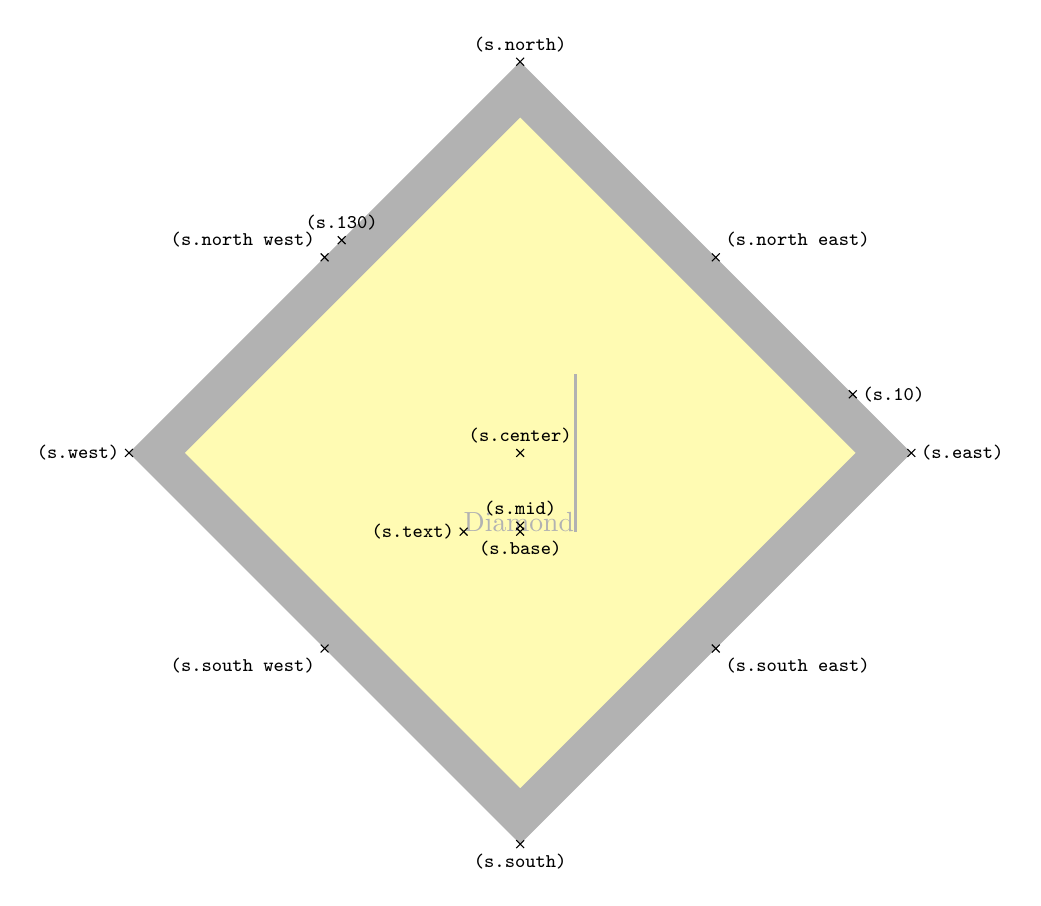
\begin{tikzpicture}
  \node[name=s,shape=diamond,shape example] {Diamond\vrule width 1pt height 2cm};
  \foreach \anchor/\placement in
    {north west/above left, north/above, north east/above right,
     west/left, center/above, east/right,
     mid/above,
     base/below,
     south west/below left, south/below, south east/below right,
     text/left, 10/right, 130/above}
     \draw[shift=(s.\anchor)] plot[mark=x] coordinates{(0,0)}
       node[\placement] {\scriptsize\texttt{(s.\anchor)}};
\end{tikzpicture}

\end{document}